\begin{figure}[H]\centering
\begin{minipage}[c]{.495\linewidth}
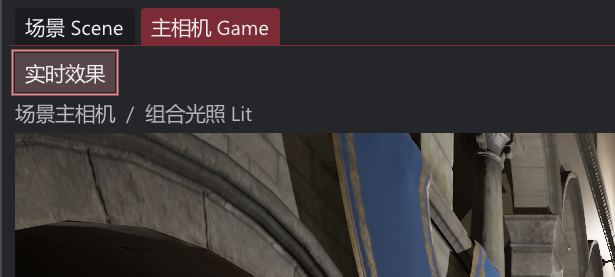
\includegraphics[width=\linewidth]{effects-button.png}
\captionline{\numtag{1}\enspace 在场景视口的工具栏点击“实时效果”。}
\end{minipage}\hfill
\begin{minipage}[c]{.44\linewidth}\centering
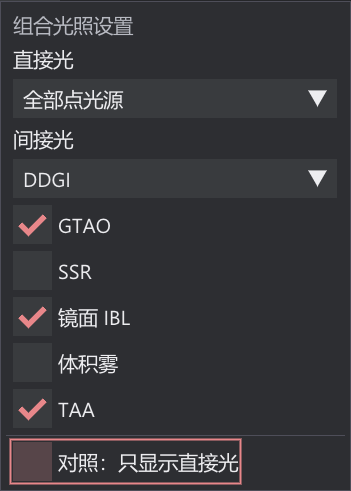
\includegraphics[height=80mm]{effects-menu.png}
\captionline{\numtag{2}\enspace 选择光照方法，勾选要叠加的效果。}
\end{minipage}
\caption{Sponza 中庭的主相机视图。图中选用全部点光源和 DDGI，已勾选 GTAO、镜面 IBL 和 TAA。SSR 与体积雾的方框为空，点击方框即可启用。}
\end{figure}
